% Created 2014-09-16 Tue 15:50
\documentclass[bigger]{beamer}
\usepackage[utf8]{inputenc}
\usepackage[T1]{fontenc}
\usepackage{fixltx2e}
\usepackage{graphicx}
\usepackage{longtable}
\usepackage{float}
\usepackage{wrapfig}
\usepackage{soul}
\usepackage{textcomp}
\usepackage{marvosym}
\usepackage{wasysym}
\usepackage{latexsym}
\usepackage{amssymb}
\usepackage{hyperref}
\tolerance=1000
\mode<beamer>{\usetheme[compress]{Berlin}}
\usepackage{graphicx}
\usepackage{amsmath}
\usepackage{lmodern}
\usepackage{ifmtarg}
\usepackage{tikz}
\usetikzlibrary{calc}
\makeatletter
\newcommand\ChangeItemFont[3]{%
\renewcommand{\itemize}[1][]{%
  \beamer@ifempty{##1}{}{\def\beamer@defaultospec{#1}}%
  \ifnum \@itemdepth >2\relax\@toodeep\else
    \advance\@itemdepth\@ne
    \beamer@computepref\@itemdepth% sets \beameritemnestingprefix
    \usebeamerfont{itemize/enumerate \beameritemnestingprefix body}%
    \usebeamercolor[fg]{itemize/enumerate \beameritemnestingprefix body}%
    \usebeamertemplate{itemize/enumerate \beameritemnestingprefix body begin}%
    \list
      {\usebeamertemplate{itemize \beameritemnestingprefix item}}
      {\def\makelabel####1{%
          {%
            \hss\llap{{%
                \usebeamerfont*{itemize \beameritemnestingprefix item}%
                \usebeamercolor[fg]{itemize \beameritemnestingprefix item}####1}}%
          }%
        }%
  \ifnum\@itemdepth=1\relax
    #1%
  \else
  \ifnum\@itemdepth=2\relax
    #2%
  \else
  \ifnum\@itemdepth=3\relax
    #3%
  \fi%
  \fi%
  \fi%
  }
  \fi%
  \beamer@cramped%
  \raggedright%
  \beamer@firstlineitemizeunskip%
}}
\makeatother


\newcommand{\doublet}[2]{
  \left(\!
    \begin{array}{c}
      {#1} \\
      {#2}
    \end{array}
    \!\right) 
}

\setbeamertemplate{footline}
  {%
    \begin{beamercolorbox}[colsep=1.5pt]{upper separation line foot}
    \end{beamercolorbox}
    \begin{beamercolorbox}[ht=2.5ex,dp=1.125ex,%
      leftskip=.3cm,rightskip=.3cm plus1fil]{author in head/foot}%
      \leavevmode{\usebeamerfont{author in head/foot}\insertshortauthor}%
      \hfill%
      {\usebeamerfont{institute in head/foot}\usebeamercolor[fg]{institute in head/foot}\insertshortinstitute}%
    \end{beamercolorbox}%
    \begin{beamercolorbox}[ht=2.5ex,dp=1.125ex,%
      leftskip=.3cm,rightskip=.3cm plus1fil]{title in head/foot}%
      {\usebeamerfont{title in head/foot}\insertshorttitle}%
      \hfill%
      {\usebeamerfont{frame number}\usebeamercolor[fg]{frame number}\insertframenumber~/~\inserttotalframenumber}
    \end{beamercolorbox}%
    \begin{beamercolorbox}[colsep=1.5pt]{lower separation line foot}
    \end{beamercolorbox}
  }
\makeatother


%--------------------------------------------------------------------------------
% Useful commands
%--------------------------------------------------------------------------------

% \urldef{\qcdurl}

%--------------------------------------------------------------------------------
% Numbers
%--------------------------------------------------------------------------------

\mode<beamer>{\usecolortheme{bear}}
\mode<beamer>{\titlegraphic{\includegraphics[width=0.2\textwidth]{brown-logo}}}
\institute[Brown University]{}
\AtBeginSection{\frame{\sectionpage}}
\providecommand{\alert}[1]{\textbf{#1}}

\title{Data Analysis Jamboree: HCAL}
\author{Edmund Berry}
\date{Tuesday, September 16, 2014}
\hypersetup{
  pdfkeywords={},
  pdfsubject={},
  pdfcreator={Emacs Org-mode version 7.9.3f}}

\author[Edmund A. Berry]{\alert{Edmund A. Berry}}
\begin{document}

\maketitle


\section{Introduction}
\label{sec-1}
\subsection{Introduction}
\label{sec-1-1}
\begin{frame}
\frametitle{Introduction}
\label{sec-1-1-1}
\begin{itemize}

\item Last few months have been very useful for HCAL
\label{sec-1-1-1-1}%

\item In addition to MWGR participation, several projects involving local running
\label{sec-1-1-1-2}%
\end{itemize} % ends low level
\begin{block}{I will focus on three major efforts:}
\label{sec-1-1-1-3}

\begin{enumerate}
\item HB sourcing
\item HF commissioning
\item Laser commissioning
\end{enumerate}
\end{block}
\end{frame}
\section{HB sourcing}
\label{sec-2}
\subsection{Introduction to sourcing}
\label{sec-2-1}
\begin{frame}
\frametitle{What is sourcing?}
\label{sec-2-1-1}
%% Figure
\label{sec-2-1-1-1}

\centering
\includegraphics[width=.9\linewidth]{fig/sourcing/sourcing_schematic.png}
\end{frame}
\begin{frame}
\frametitle{Why sourcing?}
\label{sec-2-1-2}
\begin{itemize}

\item HF: PMTs are being replaced, so sourcing old and new PMT readouts can give us first calibrations
\label{sec-2-1-2-1}%
\begin{itemize}

\item Sourcing done
\label{sec-2-1-2-1-1}%

\item Analysis ongoing
\label{sec-2-1-2-1-2}%
\end{itemize} % ends low level

\item HB/HE: Study radiation damage, comparing with sourcing before Run 1
\label{sec-2-1-2-2}%
\begin{itemize}

\item Laser in HB only probes 1 layer (9)
\label{sec-2-1-2-2-1}%

\item Laser in HE only probes 2 layers (1, 7)
\label{sec-2-1-2-2-2}%

\item Sourcing can probe all layers and look for layer-dependent radiation damage
\label{sec-2-1-2-2-3}%
\end{itemize} % ends low level

\item \alert{Focus of this discussion is HB sourcing}
\label{sec-2-1-2-3}%

\item Sourcing contact: \href{mailto:seth.cooper@cern.ch}{\underline{\alert{S. Cooper}}}
\label{sec-2-1-2-4}%

\item Analysis contact: \href{mailto:andrei.gribushin@cern.ch}{\underline{\alert{A. Gribushin}}}
\label{sec-2-1-2-5}%
\end{itemize} % ends low level
\end{frame}
\subsection{Sourcing analysis}
\label{sec-2-2}
\begin{frame}
\frametitle{Sourcing analysis}
\label{sec-2-2-1}
\begin{columns} % Columns
\label{sec-2-2-1-1}
\begin{column}{0.55\textwidth}
%% Figure 1
\label{sec-2-2-1-1-1}

\centering
Normal HF output \\(same principle for HB)
\includegraphics[width=0.8\textwidth]{fig/sourcing/sourcing_explain_1.png}
\end{column}
\begin{column}{0.55\textwidth}
%% Figure 2
\label{sec-2-2-1-1-2}

\centering
Histogram output for sourcing \\(from HCAL HTR FW)
\includegraphics[width=0.8\textwidth]{fig/sourcing/sourcing_explain_2.png}
\end{column}
\end{columns}
\begin{itemize}

\item Normally, DIGIs are read out at 40 MHz
\label{sec-2-2-1-2}%

\item Source signal is small, so fill histograms at 40 MHz \& read histograms at O(100) Hz
\label{sec-2-2-1-3}%
\end{itemize} % ends low level
\end{frame}
\begin{frame}
\frametitle{Sourcing analysis}
\label{sec-2-2-2}
\begin{columns} % Columns
\label{sec-2-2-2-1}
\begin{column}{0.55\textwidth}
%% Figure 1
\label{sec-2-2-2-1-1}

\centering
Ratio of 2005 vs. 2014 sourcing\\
from \alert{first 2014} HB sourcing
\includegraphics[width=\textwidth]{fig/sourcing/sourcing_raddam.png}
\end{column}
\begin{column}{0.55\textwidth}
%% Figure 2
\label{sec-2-2-2-1-2}

\centering
Example sourcing signal \\
from \alert{latest 2014} HB sourcing
\includegraphics[width=0.85\textwidth]{fig/sourcing/sourcing_recent.png}
\end{column}
\end{columns}
\begin{itemize}

\item First HB sourcing campaign suggests layer-dependent radiation damage of approximately 5\%
\label{sec-2-2-2-2}%

\item Latest HB sourcing campaign adds 4 more HB wedges: \alert{analysis ongoing}
\label{sec-2-2-2-3}%
\end{itemize} % ends low level
\end{frame}
\section{HF commissioning}
\label{sec-3}
\subsection{Introduction to HF improvements}
\label{sec-3-1}
\begin{frame}
\frametitle{What improvements have been made to HF?}
\label{sec-3-1-1}
\begin{itemize}

\item Why change?
\label{sec-3-1-1-1}%
\begin{itemize}

\item Punch-through
\label{sec-3-1-1-1-1}%

\item Cerenkov light in PMT glass
\label{sec-3-1-1-1-2}%
\end{itemize} % ends low level

\item What has changed already?
\label{sec-3-1-1-2}%
\begin{itemize}

\item New PMTs: thick glass \& single anode $\to$ \\ thin glass \& multi-anode
\label{sec-3-1-1-2-1}%

\item New readout cables capable of 2-channel readout
\label{sec-3-1-1-2-2}%
\end{itemize} % ends low level

\item What is still coming?
\label{sec-3-1-1-3}%
\begin{itemize}

\item Upgrade of HF backend uTCA readout (review today)
\label{sec-3-1-1-3-1}%
\end{itemize} % ends low level

\item Analysis contact: \href{mailto:katharina.bierwagen@cern.ch}{\underline{\alert{K. Bierwagen}}}
\label{sec-3-1-1-4}%
\end{itemize} % ends low level
\end{frame}
\begin{frame}
\frametitle{What improvements have been made to HF?}
\label{sec-3-1-2}
%% Figure
\label{sec-3-1-2-1}

\centering
\includegraphics[width=0.75\textwidth]{fig/hf_local/hf_commissioning.png}
\end{frame}
\subsection{HF analysis}
\label{sec-3-2}
\begin{frame}
\frametitle{HF analysis: LED gain measurement}
\label{sec-3-2-1}
\begin{columns} % Columns
\label{sec-3-2-1-1}
\begin{column}{0.55\textwidth}
%% Figure
\label{sec-3-2-1-1-1}

\centering
\includegraphics[width=.9\linewidth]{fig/hf_local/hf_gain.png}
\end{column}
\begin{column}{0.55\textwidth}
%% Text
\label{sec-3-2-1-1-2}
\begin{itemize}

\item Mean gain: \~{}127k
\label{sec-3-2-1-1-2-1}%

\item Gain RMS: \~{}12\%
\label{sec-3-2-1-1-2-2}%

\item Saturation: \~{}8 TeV
\label{sec-3-2-1-1-2-3}%
\end{itemize} % ends low level
\end{column}
\end{columns}
\end{frame}
\begin{frame}
\frametitle{PMT base board (BB) groupings}
\label{sec-3-2-2}
\begin{columns} % Columns
\label{sec-3-2-2-1}
\begin{column}{0.75\textwidth}
%% Figure 1
\label{sec-3-2-2-1-1}

\centering
\includegraphics[width=\textwidth]{fig/hf_local/hf_bb_1.png}
\end{column}
\begin{column}{0.35\textwidth}
%% Figure 2
\label{sec-3-2-2-1-2}

\centering
\includegraphics[width=\textwidth]{fig/hf_local/hf_bb_2.png}
\end{column}
\end{columns}
\end{frame}
\begin{frame}
\frametitle{HF analysis: self trigger rate}
\label{sec-3-2-3}
%% Figure 1
\label{sec-3-2-3-1}

\centering
\includegraphics[width=0.75\textwidth]{fig/hf_local/self_trigger_1.png}
%% Figure 2
\label{sec-3-2-3-2}

\centering
\includegraphics[width=0.75\textwidth]{fig/hf_local/self_trigger_2.png}
\end{frame}
\begin{frame}
\frametitle{HF analysis: after pulse rate}
\label{sec-3-2-4}
\begin{columns} % Columns
\label{sec-3-2-4-1}
\begin{column}{0.60\textwidth}
%% Text
\label{sec-3-2-4-1-1}
\begin{itemize}

\item \alert{After pulses} (APs) are spurious pulses which appear in the tail of real pulses
\label{sec-3-2-4-1-1-1}%
\begin{itemize}

\item Elastic scat. e's $\to$ \\\\
\label{sec-3-2-4-1-1-1-1}%
APs with short delays

\item Positive ions $\to$ \\\\
\label{sec-3-2-4-1-1-1-2}%
APs with long delays
\end{itemize} % ends low level

\item Look for APs within 0.25 us and 0.5 us by studying 20 TS
\label{sec-3-2-4-1-1-2}%
\begin{itemize}

\item Inject light in 1st 10 TS
\label{sec-3-2-4-1-1-2-1}%

\item Look for effect in 2nd 10 TS
\label{sec-3-2-4-1-1-2-2}%
\end{itemize} % ends low level
\end{itemize} % ends low level
\end{column}
\begin{column}{0.50\textwidth}
%% Figure
\label{sec-3-2-4-1-2}

\centering
Theoretical picture
\includegraphics[width=\textwidth]{fig/hf_local/after_pulse_intro.png}
\end{column}
\end{columns}
\end{frame}
\begin{frame}
\frametitle{HF analysis: after pulse rate}
\label{sec-3-2-5}
%% Figure 1
\label{sec-3-2-5-1}

\centering
\includegraphics[width=0.75\textwidth]{fig/hf_local/after_pulse_1.png}
%% Figure 2
\label{sec-3-2-5-2}

\centering
\includegraphics[width=0.75\textwidth]{fig/hf_local/after_pulse_2.png}
\end{frame}
\begin{frame}
\frametitle{HF analysis: rate numeric results}
\label{sec-3-2-6}
\begin{itemize}

\item Self trigger rate (thr. ET = 2 GeV):
\label{sec-3-2-6-1}%
\begin{itemize}

\item \~{}8 Hz for BB1
\label{sec-3-2-6-1-1}%

\item \~{}90 Hz for BB2
\label{sec-3-2-6-1-2}%

\item \~{}320 Hz for BB3
\label{sec-3-2-6-1-3}%
\end{itemize} % ends low level

\item After pulse rate (thr. ET = 2 GeV)
\label{sec-3-2-6-2}%
\begin{itemize}

\item \~{}0.02 Hz for BB1
\label{sec-3-2-6-2-1}%

\item \~{}1 Hz for BB2
\label{sec-3-2-6-2-2}%

\item \~{}14 Hz for BB3
\label{sec-3-2-6-2-3}%
\end{itemize} % ends low level
\end{itemize} % ends low level
\end{frame}
\section{Laser commissioning}
\label{sec-4}
\subsection{Introduction to laser commissioning}
\label{sec-4-1}
\begin{frame}
\frametitle{Introduction to laser commissioning}
\label{sec-4-1-1}
\begin{itemize}

\item HCAL laser can track radiation damage (RADDAM) in the HBHE and HF (critical in R1)
\label{sec-4-1-1-1}%

\item Laser light to megatiles excites scintillator of a particular HCAL layer
\label{sec-4-1-1-2}%

\item Laser pulse is timed to simulate actual time calorimeter signals arrive from particles produced by pp collisions at the center of CMS
\label{sec-4-1-1-3}%

\item New laser installed for 2014 to improve timing resolution
\label{sec-4-1-1-4}%

\item Analysis contact: \href{mailto:dmitry.vishnevskiy@cern.ch}{\underline{\alert{D. Vishnevskiy}}}
\label{sec-4-1-1-5}%
\end{itemize} % ends low level
\end{frame}
\subsection{Laser commissioning analysis}
\label{sec-4-2}
\begin{frame}
\frametitle{Timing improvement of new laser (HF shown)}
\label{sec-4-2-1}
\begin{columns} % Columns
\label{sec-4-2-1-1}
\begin{column}{0.55\textwidth}
%% Column 1
\label{sec-4-2-1-1-1}
%% Figure 1
\label{sec-4-2-1-1-1-1}

\centering
\includegraphics[width=\textwidth]{fig/laser/laser_2012_1.png}
%% Figure 2
\label{sec-4-2-1-1-1-2}

\centering
\includegraphics[width=\textwidth]{fig/laser/laser_2012_2.png}
\end{column}
\begin{column}{0.55\textwidth}
%% Column 2
\label{sec-4-2-1-1-2}
%% Figure 3
\label{sec-4-2-1-1-2-1}

\centering
\includegraphics[width=\textwidth]{fig/laser/laser_new.png}
\begin{itemize}

\item Old laser:\\\\
\label{sec-4-2-1-1-2-2}%
unstable timing and jitter

\item New laser: \~{}2.4 ns jitter
\label{sec-4-2-1-1-2-3}%

\item Stability is being monitored
\label{sec-4-2-1-1-2-4}%
\end{itemize} % ends low level
\end{column}
\end{columns}
\end{frame}
\begin{frame}
\frametitle{Radiation damage monitoring}
\label{sec-4-2-2}
%% Figure
\label{sec-4-2-2-1}

\centering
\includegraphics[width=0.8\textwidth]{fig/laser/hf_raddam_explanation.png}
\begin{itemize}

\item Principle of RADDAM monitoring is to measure S1/S2
\label{sec-4-2-2-2}%

\item S1/S2 varies as a function of phase (laser - TTC)
\label{sec-4-2-2-3}%

\item Need to find a region of phase where S1/S2 is stable
\label{sec-4-2-2-4}%
\end{itemize} % ends low level
\end{frame}
\begin{frame}
\frametitle{Phase scan needed}
\label{sec-4-2-3}
%% Figure
\label{sec-4-2-3-1}

\centering
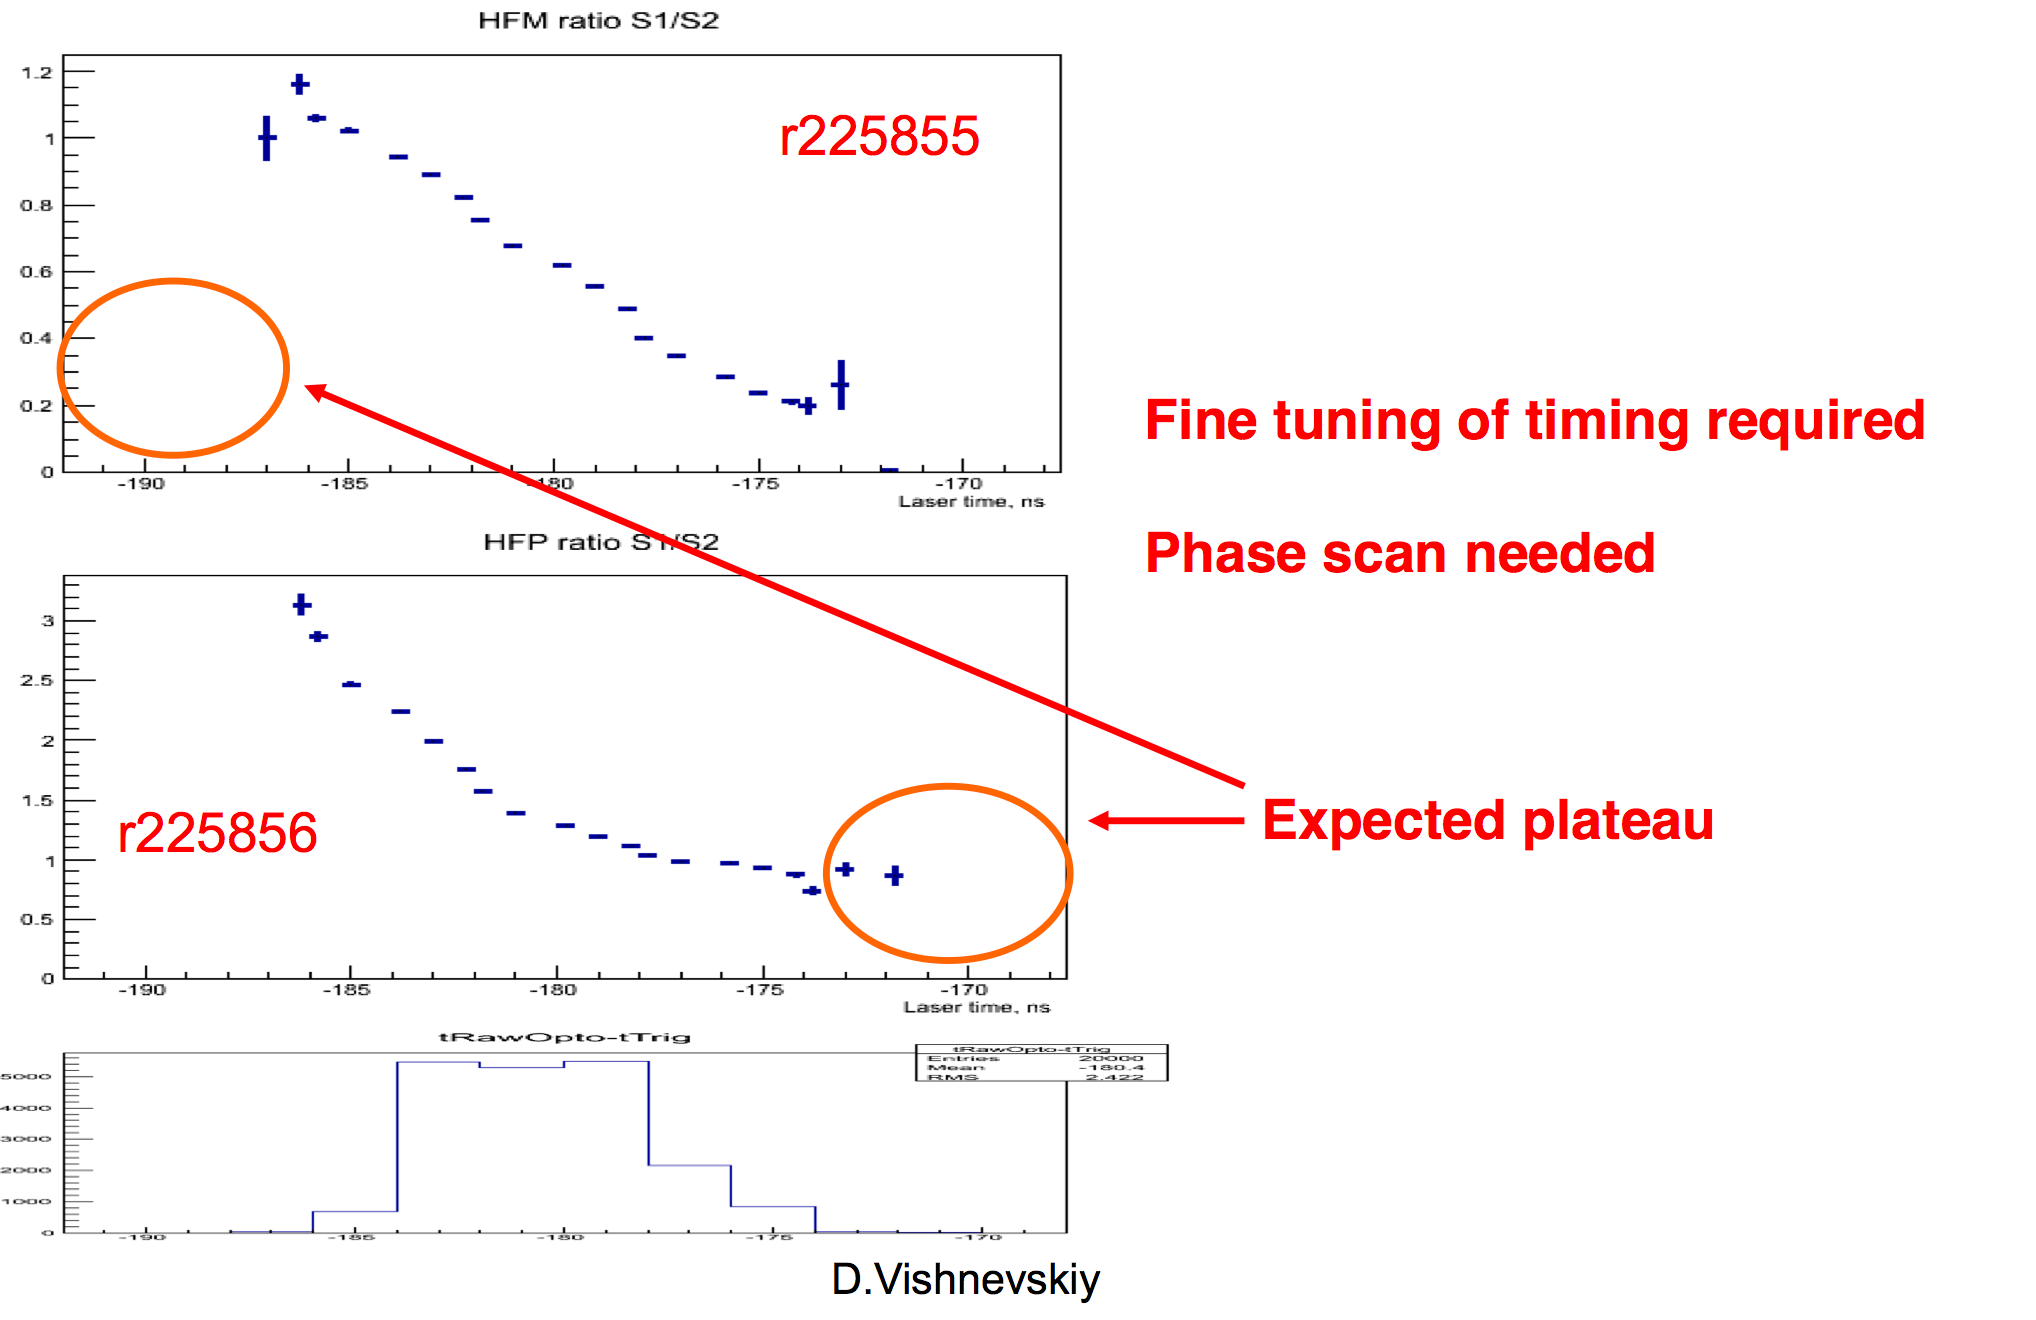
\includegraphics[width=0.8\textwidth]{fig/laser/laser_plateau.png}
\begin{itemize}

\item Lack of plateau region shows laser is not timed in
\label{sec-4-2-3-2}%

\item Phase scan needed
\label{sec-4-2-3-3}%
\end{itemize} % ends low level
\end{frame}
\section{Conclusion}
\label{sec-5}
\subsection{To-do list \& Conclusion}
\label{sec-5-1}
\begin{frame}
\frametitle{Partial to-do list}
\label{sec-5-1-1}

\begin{enumerate}
\item Complete sourcing analysis
\begin{itemize}
\item start-up calibration of HF
\item better understanding of radiation damage in HBHE
\end{itemize}
\item Complete commissioning of Laser
\item Continue taking/analyzing reg. local commissioning runs
\end{enumerate}
\end{frame}
\begin{frame}
\frametitle{Conclusion}
\label{sec-5-1-2}
\begin{itemize}

\item HCAL has been very busy over the last few months
\label{sec-5-1-2-1}%

\item These slides discuss three important campaigns \\ (among others):
\label{sec-5-1-2-2}%
\begin{itemize}

\item Analysis of HB sourcing data has already yielded interesting results.  More analysis is coming.
\label{sec-5-1-2-2-1}%

\item HF installation and commissioning is finalized, and basic detector parameters have been established.  These include two PMT effects, which contribute  extra energy to the event
\label{sec-5-1-2-2-2}%

\item A new laser with significantly improved timing resolution is being commissioned
\label{sec-5-1-2-2-3}%
\end{itemize} % ends low level
\end{itemize} % ends low level
\end{frame}

\end{document}
